% !TeX encoding = UTF-8
% Do not touch the below 70 lines
\documentclass[11pt,a4paper,onecolumn,oneside]{report}

\usepackage{mathptmx}
\usepackage[T1]{fontenc}
\usepackage[utf8]{inputenc}

\RequirePackage[top=3cm, bottom=1in, left=1in, right=1in]{geometry}
\linespread{1.3}

\usepackage{titlesec}
\usepackage{amsmath}
\usepackage{amssymb}
\usepackage{mathtools}
\usepackage{enumerate}
\usepackage{bbm}
\usepackage{algorithm}
\usepackage{algorithmic}
\usepackage{epsfig}
\usepackage{color}
\usepackage{graphicx}
\usepackage{caption}
\usepackage{subcaption}
\usepackage{cases}
\usepackage{url}
\usepackage{cite}
\usepackage{fancyhdr}
\usepackage{tocloft}
\usepackage{pdfpages}

\renewcommand\cftsecafterpnum{\vskip15pt}
\renewcommand\cftsubsecafterpnum{\vskip15pt}
\renewcommand\cftfigafterpnum{\vskip15pt}
\renewcommand{\thesection}{\Roman{section}}
\renewcommand{\thesubsection}{\arabic{section}.\arabic{subsection}}
\renewcommand{\contentsname}{\hfill\bfseries\Large Contents\hfill}
\renewcommand{\listfigurename}{\hfill\bfseries\Large List of Figures\hfill}
\renewcommand{\thefigure}{\arabic{figure}}
\newcommand{\qed}{\hfill\blacksquare}
\renewcommand{\bibname}{\hfill\bfseries\Large References \hfill\hfill}
\renewcommand{\abstractname}{\bfseries\Large Abstract \hfill\hfill}

\newcounter{lemma}
\newcounter{proposition}
\newcounter{theorem}
\newtheorem{lemma}{\bf Lemma}
\newtheorem{proposition}{\bf Proposition}
\newtheorem{theorem}{\bf Theorem}
\newtheorem{proof}{\bf Proof}

%\input{mymath_mod.tex}

\newcommand{\HIGH}[1]{{\textcolor{blue}{#1}}}
%\renewcommand{\baselinestretch}{1.5}

\DeclareMathOperator*{\argmax}{arg\,max}

\fancyhf{}
\renewcommand{\headrulewidth}{0pt}
\cfoot{\thepage}
\pagestyle{fancy}
%\pagenumbering{gobble}

% Do not touch the above 70 lines

\begin{document}

% Front cover
    \begin{center}
    \LARGE Doctoral Thesis

    \vspace{3cm}
    \huge <Title>
    % Great Work That None Can Do Except Me

    \vfill

    \LARGE Jaewoong Lee

    \vspace{2cm}

    \LARGE Department of Biomedical Engineering

    \LARGE (<Your major>)
    % (Check your major. Write only if your major name is different from your department(school))

    \vspace{2cm}

    \LARGE Ulsan National Institute of Science and Technology
    \vspace{2cm}

    \LARGE \the\year{}

    \end{center}
    \thispagestyle{empty}
    \clearpage

% Title page
    \begin{center}
    \hbox{ }

    \hbox{ }

    \huge <Title>
    % Great Work That None Can Do Except Me

    \vspace{5cm}

    \LARGE <Your name>
    % Gil Dong Hong

    \vspace{6cm}

    \LARGE <Your department>
    % Department of Computer Science and Engineering

    \LARGE (<Your major>)
    % Check your major. Write only if your major name is different from your department(school)

    \vspace{2cm}

    \LARGE Ulsan National Institute of Science and Technology

    \end{center}
    \thispagestyle{empty}
    \clearpage

% Thesis approval
% Add the approval doc signed by your advisor in a PDF file
% Put your pdf with the filename below, and uncomment it.
    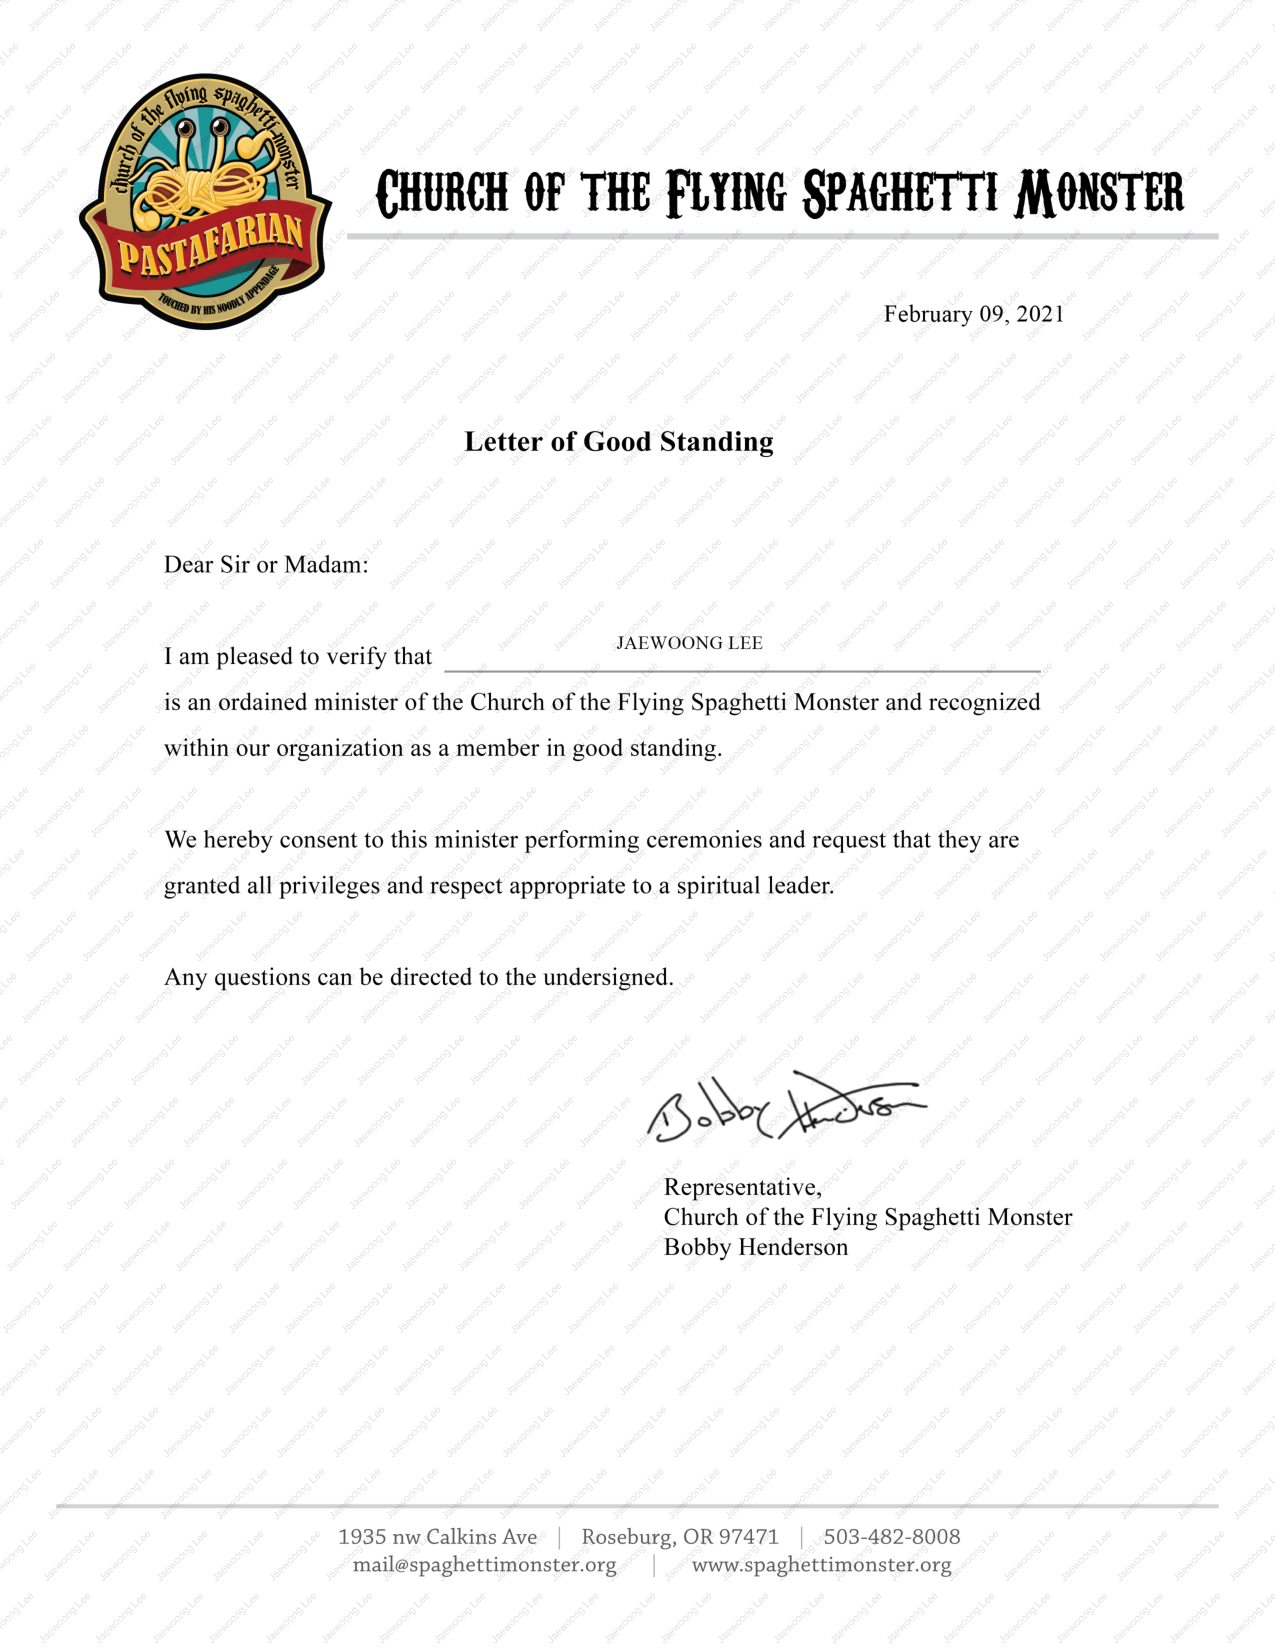
\includepdf[fitpaper= true, pages=-]{Documents/example.pdf}

% [Confirmation of thesis approval]
% add the certificate signed by your committee in a PDF file
% Put your pdf with the filename below, and uncomment it.
    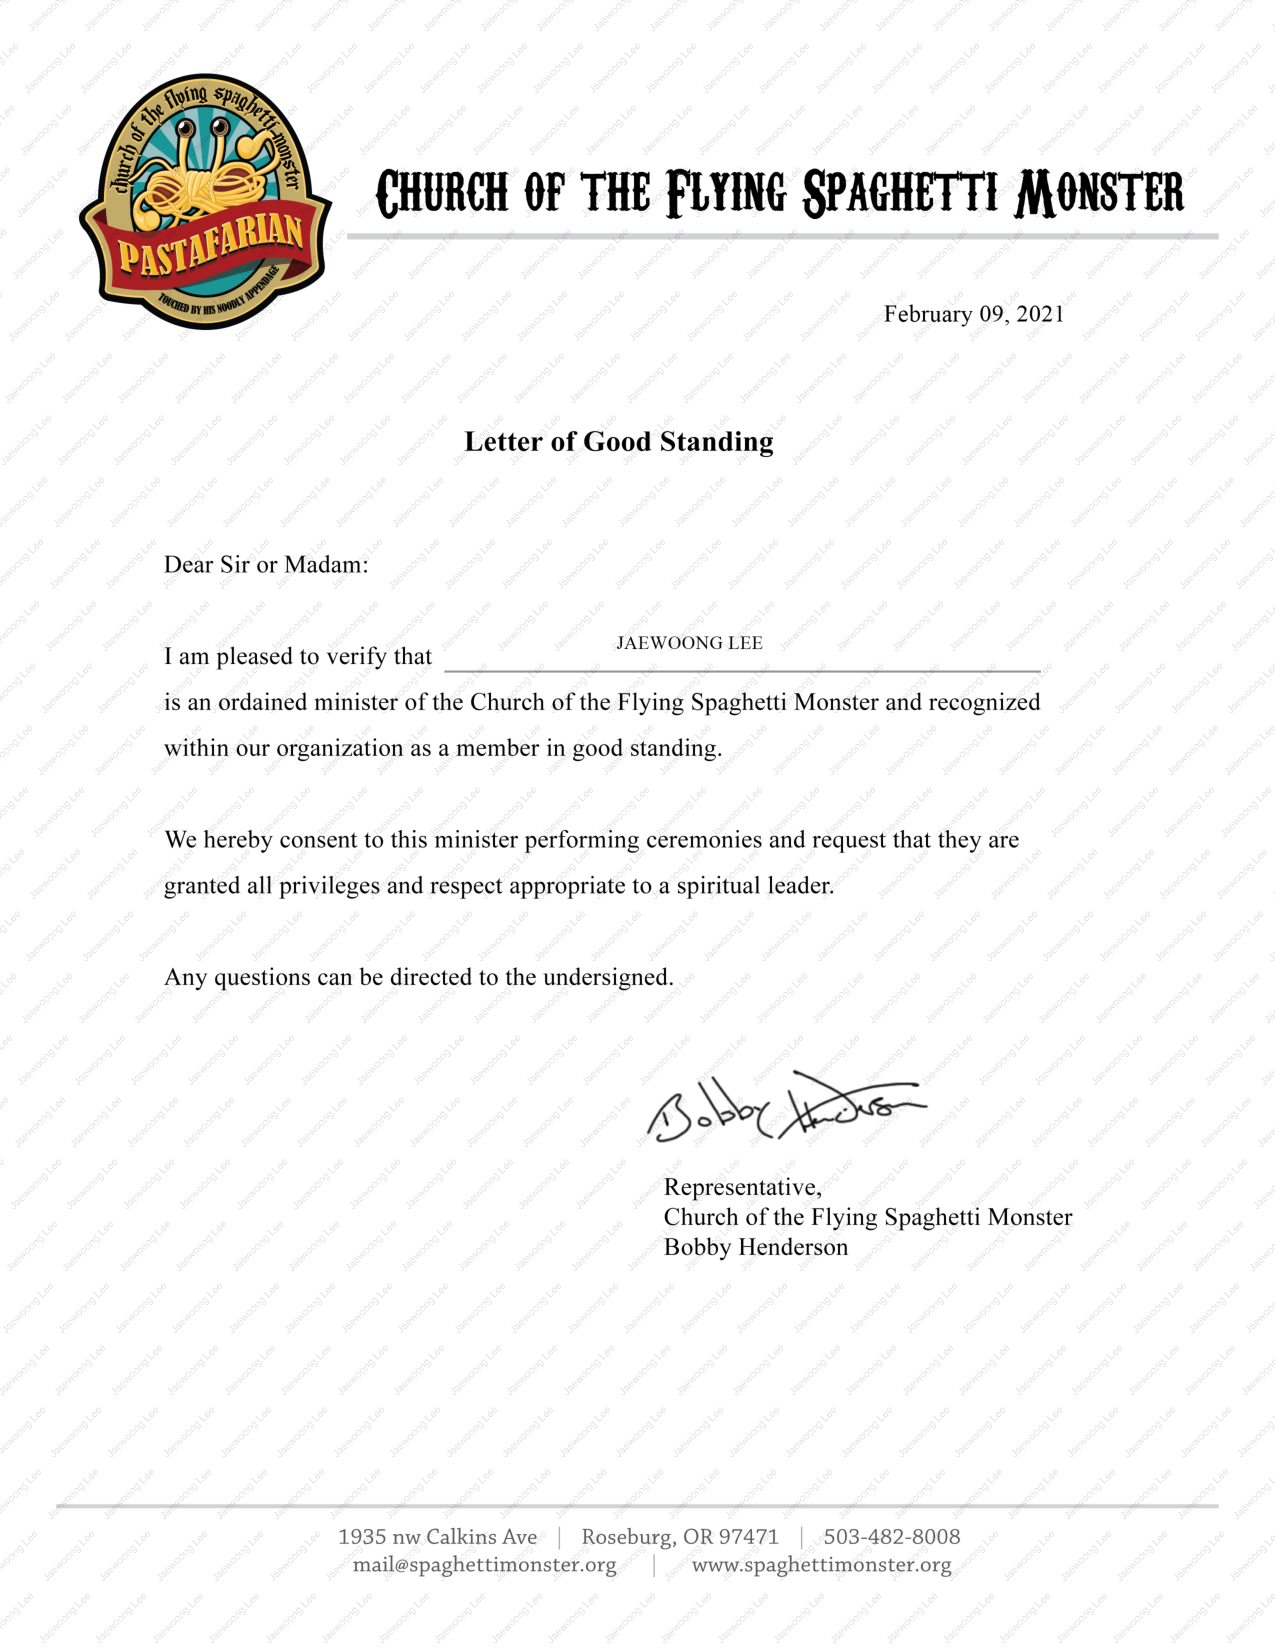
\includepdf[fitpaper= true, pages=-]{Documents/example.pdf}

% Abstract
    \begin{abstract}
    Your abstract should be here. \vfill
    \end{abstract}

\clearpage

% Do not touch the below 20 lines
\hbox{ }
\thispagestyle{empty}
\clearpage

%%% Table of Contents
\tableofcontents{}
\thispagestyle{empty}
\vfill
\clearpage

%%% List of Figures
\listoffigures{}
\thispagestyle{empty}
\clearpage

%%% reset page numbering
\setcounter{page}{1}
%  Do not touch the above 20 lines

    \section*{List of abbreviations}
    \newpage

    \section{Introduction}

        Your introduction should be here. You may need a reference~\cite{ref_sample}.
    \newpage

    \section{Second section}
        My second section starts with my equation, which can be written as

        \begin{equation}\label{eq:myeq}
        \begin{split}
        	A 		&= B + C, \\
            D + E	&= F.
        \end{split}
        \end{equation}
        Thus we have (\ref{eq:myeq}).

        Fig.~\ref{fig:myfigure} is a sample figure.

        \begin{figure}[h]
        \centering
        
\includegraphics[width=12 cm]{Figures/myfigure.pdf}
        \caption{My figure.} \label{fig:myfigure}
        \end{figure}
    \newpage

    \section{Third section}
    My third section starts.

        \subsection{First subsection}
            This is the first subsection.


            \begin{algorithm}
            	\caption{My Algorithm.} \label{algo:myalgo}
                At the beginning ...

            	\begin{algorithmic}[1]
            	    \STATE Do this
                    \STATE and do this\\
                    /* add explanation if necessary */
                    \STATE Finally do this
            	\end{algorithmic}
            \end{algorithm}

            Algorithm~\ref{algo:myalgo} is our proposed algorithm.

        \subsection{Another subsection}
    \newpage

    \section{Following Sections}
    \newpage

    \section{Conclusion}
        My conclusion here.
    \clearpage

% Reference
    \addcontentsline{toc}{section}{References}
    \bibliographystyle{IEEEtran}
    \bibliography{sample.bib}
    \clearpage


% Acknowledgements
    \addcontentsline{toc}{section}{Acknowledgments}
    \section*{\hfill \Large Acknowledgments \hfill}
        Thank you very much.
    \clearpage

%%% The following page is intentionally left as blank
% White attachment form
\hbox{ }
\thispagestyle{empty}
\clearpage

\end{document}